% !TEX root = ../../STP_IoTjournal.tex
\subsection{Setup \label{sec:bayArea_simSetup}}
We grid the San Francisco Bay Area in California, US and use it as our state space, as shown in Figure \ref{fig:bayArea_setup}. We consider the UAVs flying to and from four cities: Richmond, Berkeley, Oakland, and San Francisco. The blue region in Fig. \ref{fig:bayArea_setup} represents bay. This environment is different from the city environment in Section \ref{sec:city_sim} in that now the UAVs need to fly for longer distances and through a high-density vehicle environment with strong winds, but have very few static obstacles like tall buildings.    
%
\begin{figure}
  \centering
  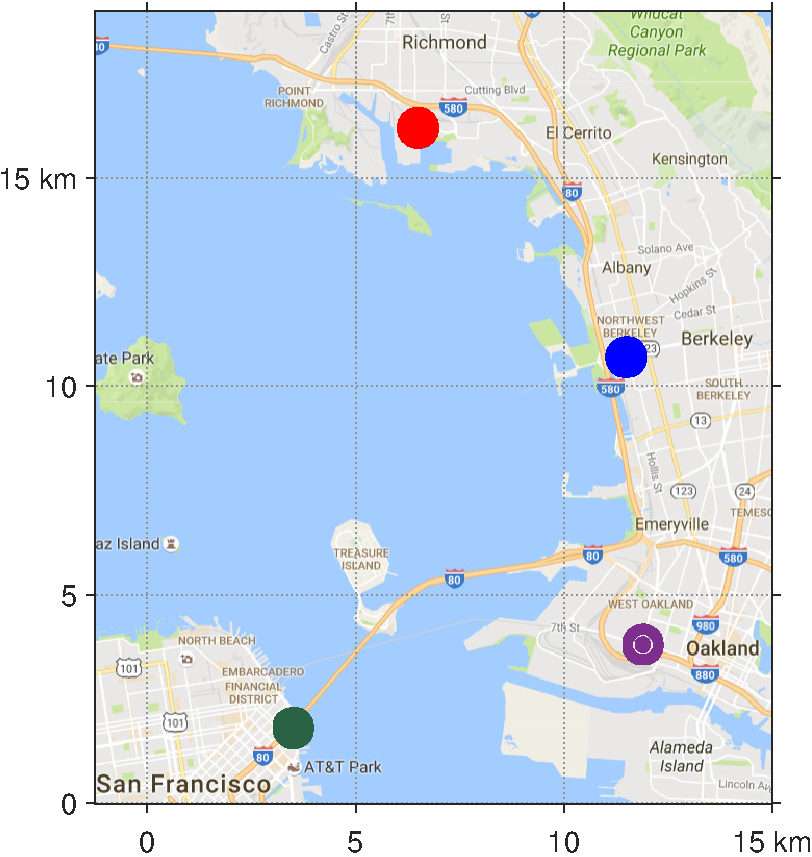
\includegraphics[width=\columnwidth]{figs/bayArea_setup}
  \caption{Multi-city simulation setup. A $300 km^2$ area of San Francisco Bay Area is used as the state-space for vehicles. STP vehicles fly to and from the four cities indicated by the four circles. The simulations are performed under the strong winds condition with $d_{r} = 11 m/s$.}
  \label{fig:bayArea_setup}
\end{figure}

Each box in Figure \ref{fig:bayArea_setup} represents a $25$ km$^2$ area. The vehicles are flying to and from the four cities indicated by the four circles. The origin and the destination of each vehicle is chosen randomly from these four cities. The vehicle dynamics are given by \eqref{eq:dyn_i}. We choose velocity and turn-rate bounds as $\underline{v} = 0$ m/s, $\bar{v} = 25$ m/s, $\bar\omega = 2$ rad/s. The disturbance bound is chosen as $d_{r} = 11$ m/s, which corresponds to \textit{strong breeze} on Beaufort wind force scale \cite{Windscale}. The scheduled time of arrival $\sta$ for vehicles are chosen as $5(i-1)$ s.

The goal of the vehicles is to reach their destinations while avoiding a collision with the other vehicles. The joint state space of this 200-vehicle system is 600-dimensional, making the joint trajectory planning and collision avoidance problem intractable for direct analysis. Therefore, we assign a priority order to vehicles and solve the trajectory planning problem sequentially.